\chapter{Polímeros: síntesis, estructura y propiedades}\label{ch:b2:polymer-synthesis}

Las medias de nailon salieron a la venta en 1939. Procedían de un laboratorio que se había propuesto, unos años
antes, comprender cómo se unen las moléculas pequeñas para formar moléculas largas, y que por el camino había aprendido una
lección que sorprende a todo químico la primera vez: para un \omterm{def:b2:polymer-synthesis:polymer}{polímero} formado uniendo moléculas extremo con extremo,
un rendimiento del 99~\% no basta. Este capítulo explica por qué, describe las dos maneras en que crecen las cadenas
y relaciona la estructura de las cadenas con las propiedades de los materiales.
% ledger: hist:nylon-production-1939

\begin{recall}
El volumen escolar: \omterm{def:b2:polymer-synthesis:polymer}{polímeros}, \omterm{def:b2:polymer-synthesis:polymer}{monómeros} y \omterm{def:b2:polymer-synthesis:polymer}{unidades de repetición}, \omterm{def:b2:polymer-synthesis:polymer}{polímeros} de adición y de condensación,
termoplásticos y termoestables. El volumen del primer año: radicales y homólisis, carbocationes y
carbaniones, aproximación del estado estacionario. \Cref{ch:b2:acyl-substitution}: ésteres y amidas.
\Cref{ch:b2:catalytic-cycles}: inserción en un enlace metal--carbono.
\end{recall}

\section{Las cadenas y sus masas molares}

\begin{definition}[Polímero]\label{def:b2:polymer-synthesis:polymer}
Un \emph{polímero}\index{polimero@polímero} es una sustancia formada por macromoléculas, cada una construida por la unión
repetida de moléculas pequeñas, los \emph{monómeros}\index{monomero@monómero}. La \emph{unidad de repetición}\index{unidad de repeticion@unidad de repetición}
es el grupo de átomos más pequeño cuya repetición forma la cadena; el \emph{grado de
polimerización}\index{grado de polimerizacion@grado de polimerización} $X$ de una cadena es el número de unidades procedentes de monómeros
que contiene.
\end{definition}

Una muestra de un \omterm{def:b2:polymer-synthesis:polymer}{polímero} sintético nunca está formada por cadenas idénticas: es una mezcla de cadenas de
longitudes distintas, y su masa molar es una media, que depende de cómo se cuenten las cadenas.

\begin{definition}[Masas molares medias]\label{def:b2:polymer-synthesis:averages}
Para una muestra que contiene $N_i$ cadenas de masa molar $M_i$, la \emph{masa molar media en
número}\index{masa molar media en numero@masa molar media en número} y la \emph{masa molar media en masa}\index{masa molar media en masa}
son
\begin{equation*}
\bar M_n = \frac{\sum_i N_i M_i}{\sum_i N_i}, \qquad
\bar M_w = \frac{\sum_i N_i M_i^2}{\sum_i N_i M_i} = \sum_i w_i M_i,
\end{equation*}
donde $w_i$ es la fracción másica de las cadenas de masa $M_i$. La \emph{dispersidad}\index{dispersidad}
$\text{\DH} = \bar M_w/\bar M_n$ es como mínimo 1, e igual a 1 solo si todas las cadenas tienen la misma
masa. Las medias $\bar X_n$ y $\bar X_w$ del \omterm{def:b2:polymer-synthesis:polymer}{grado de polimerización} se definen del mismo
modo.
\end{definition}

La media en número pondera cada cadena una vez; la media en masa pondera cada cadena por su masa, de modo que las
cadenas largas cuentan más. Que $\text{\DH} \ge 1$ es la desigualdad $\left(\sum N_i M_i\right)^2 \le
\sum N_i \sum N_i M_i^2$ (Cauchy--Schwarz), con igualdad solo si todas las $M_i$ son iguales.

\begin{method}[Calcular las medias]\label{met:b2:polymer-synthesis:averages}
\begin{enumerate}
  \item Conviértanse los datos en cantidades $N_i$ (o números de cadenas) y masas $M_i$; a partir de fracciones másicas,
        $N_i \propto w_i/M_i$.
  \item $\bar M_n = \sum N_i M_i / \sum N_i$; de forma equivalente, $1/\bar M_n = \sum w_i/M_i$.
  \item $\bar M_w = \sum w_i M_i$.
  \item $\text{\DH} = \bar M_w/\bar M_n$; compruébese que $\bar M_w \ge \bar M_n$.
\end{enumerate}
\end{method}

\section{Crecimiento por etapas y crecimiento en cadena}

\begin{definition}[Crecimiento por etapas y en cadena]\label{def:b2:polymer-synthesis:step-chain}
En una \emph{polimerización por etapas}\index{polimerizacion por etapas@polimerización por etapas}, dos moléculas cualesquiera que lleven
grupos funcionales complementarios (\omterm{def:b2:polymer-synthesis:polymer}{monómeros}, oligómeros o cadenas largas) pueden reaccionar, y las cadenas
se alargan uniéndose unas con otras: poliésteres, poliamidas. En una \emph{polimerización en
cadena}\index{polimerizacion en cadena@polimerización en cadena}, un centro reactivo (radical, ion o enlace metal--carbono)
adiciona moléculas de \omterm{def:b2:polymer-synthesis:polymer}{monómero} de una en una al extremo de una cadena en crecimiento: los \omterm{def:b2:polymer-synthesis:polymer}{polímeros} de los alquenos.
\end{definition}

\begin{method}[¿Por etapas o en cadena?]\label{met:b2:polymer-synthesis:classify}
\begin{enumerate}
  \item Un \omterm{def:b2:polymer-synthesis:polymer}{monómero} con dos grupos funcionales que reaccionan cada uno con el compañero del otro (ácido y alcohol,
        ácido y amina), a menudo con liberación de una molécula pequeña: crecimiento por etapas.
  \item Un \omterm{def:b2:polymer-synthesis:polymer}{monómero} con un doble enlace \ce{C=C} (o un anillo tensionado) y un iniciador: crecimiento en cadena.
  \item Compruébese con el curso de la reacción: en el crecimiento por etapas, el \omterm{def:b2:polymer-synthesis:polymer}{monómero} desaparece pronto y las cadenas largas
        solo aparecen al final; en el crecimiento en cadena, las cadenas largas aparecen desde el principio mientras el \omterm{def:b2:polymer-synthesis:polymer}{monómero}
        se consume gradualmente.
\end{enumerate}
\end{method}

\subsection*{Crecimiento por etapas}

Tómese una mezcla equilibrada de \omterm{def:b2:polymer-synthesis:polymer}{monómeros} \ce{A-A} y \ce{B-B} (una diamina y un diácido), o un único
\omterm{def:b2:polymer-synthesis:polymer}{monómero} \ce{A-B}. Llámese $p$ el \emph{grado de avance}: la fracción de los grupos funcionales de un
tipo que han reaccionado.

\begin{theorem}[Ecuación de Carothers]\label{thm:b2:polymer-synthesis:carothers}
En una \omterm{def:b2:polymer-synthesis:step-chain}{polimerización por etapas} de \omterm{def:b2:polymer-synthesis:polymer}{monómeros} bifuncionales exactamente equilibrados, el \omterm{def:b2:polymer-synthesis:polymer}{grado de polimerización} medio en
número, contado en unidades monoméricas, es
\begin{equation*}
\bar X_n = \frac{1}{1 - p}.
\end{equation*}
\end{theorem}

\begin{proof}
Partamos de $N_0$ moléculas de \omterm{def:b2:polymer-synthesis:polymer}{monómero}, que llevan $N_0$ grupos \ce{A} y $N_0$ grupos \ce{B}. Cada reacción
entre un \ce{A} y un \ce{B} une dos moléculas en una, de modo que reduce en uno el número de moléculas.
Tras $pN_0$ reacciones quedan $N = N_0 - pN_0 = N_0(1-p)$ moléculas que se reparten las $N_0$ unidades
monoméricas: $\bar X_n = N_0/N = 1/(1-p)$.
\end{proof}

\begin{corollary}[Desequilibrio]\label{cor:b2:polymer-synthesis:imbalance}
Si los grupos no están equilibrados, con $r = N_{\ce{A}}/N_{\ce{B}} \le 1$ y $p$ el grado de avance de
los grupos minoritarios \ce{A},
\begin{equation*}
\bar X_n = \frac{1 + r}{1 + r - 2rp}, \qquad \text{como máximo } \frac{1+r}{1-r} \text{ cuando } p = 1.
\end{equation*}
\end{corollary}

\begin{proof}
Al principio hay $(N_{\ce{A}} + N_{\ce{B}})/2$ moléculas de \omterm{def:b2:polymer-synthesis:polymer}{monómero} bifuncional. Cada molécula
lineal tiene dos extremos de cadena, cada uno un grupo sin reaccionar; tras la reacción quedan $N_{\ce{A}}(1-p)$
grupos \ce{A} y $N_{\ce{B}} - pN_{\ce{A}}$ grupos \ce{B}, luego $N = [N_{\ce{A}}(1-p) + N_{\ce{B}} -
pN_{\ce{A}}]/2$ moléculas. Dividiendo, con $N_{\ce{B}} = N_{\ce{A}}/r$:
$\bar X_n = (1 + 1/r)/(1 - 2p + 1/r) = (1+r)/(1 + r - 2rp)$. Con $r = 1$ se recupera la ecuación de Carothers.
\end{proof}

La ecuación explica el enigma inicial. Para $p = 0.99$, un ``rendimiento del 99~\%'' de la reacción de unión, $\bar X_n =
100$; una fibra útil necesita eso o más, de modo que la unión debe superar el 99~\%, con \omterm{def:b2:polymer-synthesis:polymer}{monómeros} puros
en cantidades exactamente iguales y eliminando la molécula pequeña liberada (agua, metanol) para seguir desplazando el
equilibrio. Un exceso del 1~\% de uno de los \omterm{def:b2:polymer-synthesis:polymer}{monómeros} limita $\bar X_n$ a 201 incluso con \omterm{def:b2:continuous-reactors:conversion}{conversión} completa.

\begin{theorem}[Distribución de Flory]\label{thm:b2:polymer-synthesis:flory}
En una \omterm{def:b2:polymer-synthesis:step-chain}{polimerización por etapas} con grado de avance $p$, si todos los grupos tienen la misma reactividad sea cual sea la
longitud de su cadena, la fracción en número y la fracción másica de las cadenas de $x$ unidades son
\begin{equation*}
n_x = (1-p)\,p^{\,x-1}, \qquad w_x = x(1-p)^2 p^{\,x-1},
\end{equation*}
y $\bar X_n = 1/(1-p)$, $\bar X_w = (1+p)/(1-p)$, de modo que $\text{\DH} = 1 + p$, cercana a 2 a \omterm{def:b2:continuous-reactors:conversion}{conversión}
elevada.
\end{theorem}

\begin{proof}
Sígase una cadena desde un extremo (un \omterm{def:b2:polymer-synthesis:polymer}{monómero} \ce{A-B}, por simplicidad). Cada enlace a lo largo de ella se forma con
probabilidad $p$, de forma independiente. La cadena tiene exactamente $x$ unidades si los $x-1$ primeros enlaces se forman
y el siguiente no: probabilidad $p^{\,x-1}(1-p)$, que es $n_x$. Con $\sum_{x\ge1} p^{\,x-1} =
1/(1-p)$ y sus derivadas $\sum x p^{\,x-1} = 1/(1-p)^2$ y $\sum x^2 p^{\,x-1} = (1+p)/(1-p)^3$:
$\sum n_x = 1$, $\bar X_n = \sum x n_x = 1/(1-p)$, $w_x = x n_x/\bar X_n = x(1-p)^2p^{\,x-1}$, y
$\bar X_w = \sum x w_x = (1-p)^2(1+p)/(1-p)^3 = (1+p)/(1-p)$.
\end{proof}

\begin{omfigure}
\begin{tikzpicture}
\begin{axis}[width=0.46\linewidth, height=5cm, xmin=0, xmax=400, ymin=0,
  xlabel={grado de polimerización $x$}, ylabel={fracción másica $w_x$}, label style={font=\small},
  tick label style={font=\scriptsize}, scaled y ticks=false,
  yticklabel style={/pgf/number format/fixed, /pgf/number format/precision=3},
  legend style={font=\scriptsize, at={(0.98,0.98)}, anchor=north east}, legend cell align=left]
\addplot[omDef, thick] table[x=x, y=p95] {figdata/out/bachelor-2-polymer-distributions-a.dat};
\addplot[omThm, thick] table[x=x, y=p98] {figdata/out/bachelor-2-polymer-distributions-a.dat};
\addplot[omMeth, thick] table[x=x, y=p99] {figdata/out/bachelor-2-polymer-distributions-a.dat};
\legend{$p = 0.95$, $p = 0.98$, $p = 0.99$}
\end{axis}
\end{tikzpicture}\hfill
\begin{tikzpicture}
\begin{axis}[width=0.46\linewidth, height=5cm, xmin=0, xmax=1, ymin=0, ymax=200,
  xlabel={grado de avance $p$}, ylabel={$\bar X_n$}, label style={font=\small},
  tick label style={font=\scriptsize}, xtick={0,0.2,0.4,0.6,0.8,1}]
\addplot[omDef, thick] table[x=p, y=Xn] {figdata/out/bachelor-2-polymer-distributions-b.dat};
\end{axis}
\end{tikzpicture}

{\small \omterm{def:b2:polymer-synthesis:step-chain}{Polimerización por etapas} (modelos). Izquierda: distribuciones másicas de Flory
(\cref{thm:b2:polymer-synthesis:flory}); el máximo se sitúa cerca de $\bar X_n$ y la distribución se ensancha a medida que
se desplaza. Derecha: la ecuación de Carothers; $\bar X_n$ sigue siendo pequeño hasta que $p$ está muy cerca de 1.}
% figdata: bachelor-2/polymer-distributions.py parts a, b
\end{omfigure}

\subsection*{Crecimiento radicalario en cadena}

\begin{definition}[Etapas de una polimerización en cadena]\label{def:b2:polymer-synthesis:chain-steps}
Una polimerización radicalaria en cadena transcurre en tres tipos de etapas. En la \emph{iniciación}\index{iniciacion@iniciación}, un
\emph{iniciador radicalario}\index{iniciador radicalario} (una molécula con un enlace débil, como un peróxido o un
compuesto azoico) se escinde al calentarse en radicales, uno de los cuales se adiciona a un \omterm{def:b2:polymer-synthesis:polymer}{monómero}. En la
\emph{propagación}\index{propagacion@propagación}, el radical del extremo de la cadena adiciona una molécula de \omterm{def:b2:polymer-synthesis:polymer}{monómero} y sigue siendo
un radical. En la \emph{terminación}\index{terminacion@terminación}, dos radicales se destruyen mutuamente, por combinación
(se unen) o por desproporción (uno toma un átomo de hidrógeno del otro).
\end{definition}

\begin{omfigure}
\begin{align*}
&\text{iniciación:} && \mathrm{I{-}I} \longrightarrow 2\,\mathrm{I^{\bullet}}, \qquad
\mathrm{I^{\bullet} + CH_2{=}CHPh \longrightarrow I{-}CH_2{-}\dot{C}HPh} \\
&\text{propagación:} && {\sim}\mathrm{CH_2{-}\dot{C}HPh + CH_2{=}CHPh \longrightarrow}\;
{\sim}\mathrm{CH_2{-}CHPh{-}CH_2{-}\dot{C}HPh} \\
&\text{terminación:} && {\sim}\mathrm{CH_2{-}\dot{C}HPh + Ph\dot{C}H{-}CH_2}{\sim} \longrightarrow
{\sim}\mathrm{CH_2{-}CHPh{-}CHPh{-}CH_2}{\sim}
\end{align*}

{\small Polimerización radicalaria del estireno. El iniciador \ce{I-I} (el peróxido de dibenzoílo, por ejemplo)
se escinde en dos radicales; cada uno se adiciona al extremo \ce{CH2} del estireno, dando el radical
bencílico, más estable; la \omterm{def:b2:polymer-synthesis:chain-steps}{propagación} repite la adición miles de veces; dos radicales de cadena se combinan y terminan ambas
cadenas. El punto señala el electrón desapareado.}
\end{omfigure}

\begin{theorem}[Velocidad de la polimerización radicalaria]\label{thm:b2:polymer-synthesis:radical-rate}
Con un iniciador que se descompone con constante de velocidad $k_d$ y eficacia $f$ (la fracción de radicales que
inician una cadena), una constante de \omterm{def:b2:polymer-synthesis:chain-steps}{propagación} $k_p$ y una constante de \omterm{def:b2:polymer-synthesis:chain-steps}{terminación} $k_t$ (velocidad de \omterm{def:b2:polymer-synthesis:chain-steps}{terminación} $2k_t
[\mathrm{M^\bullet}]^2$), la velocidad de polimerización en régimen estacionario es
\begin{equation*}
R_p = k_p [\mathrm M] \sqrt{\frac{f k_d [\mathrm I]}{k_t}}.
\end{equation*}
\end{theorem}

\begin{proof}
Sea $[\mathrm{M^\bullet}]$ la concentración total de radicales de cadena, sea cual sea su longitud. Se
crean con la velocidad $R_i = 2fk_d[\mathrm I]$ (dos radicales por molécula de iniciador, de los que una fracción $f$
inicia cadenas) y se destruyen con la velocidad $2k_t[\mathrm{M^\bullet}]^2$; la \omterm{def:b2:polymer-synthesis:chain-steps}{propagación} convierte un radical de cadena
en otro y no cambia su número. La aproximación del estado estacionario aplicada a
$[\mathrm{M^\bullet}]$ da $2fk_d[\mathrm I] = 2k_t[\mathrm{M^\bullet}]^2$, luego $[\mathrm{M^\bullet}] =
\sqrt{fk_d[\mathrm I]/k_t}$. El \omterm{def:b2:polymer-synthesis:polymer}{monómero} se consume esencialmente por \omterm{def:b2:polymer-synthesis:chain-steps}{propagación}, a $R_p =
k_p[\mathrm M][\mathrm{M^\bullet}]$.
\end{proof}

\begin{definition}[Longitud de cadena cinética]\label{def:b2:polymer-synthesis:chain-length}
La \emph{longitud de cadena cinética}\index{longitud de cadena cinetica@longitud de cadena cinética} $\nu$ es el número medio de moléculas de \omterm{def:b2:polymer-synthesis:polymer}{monómero}
adicionadas por cada radical que inicia una cadena: $\nu = R_p/R_i$.
\end{definition}

\begin{proposition}[Longitud de cadena e iniciador]\label{prop:b2:polymer-synthesis:chain-length}
En régimen estacionario, $\nu = k_p[\mathrm M]/\bigl(2\sqrt{fk_dk_t[\mathrm I]}\bigr)$: más iniciador da una
polimerización más rápida pero cadenas más cortas. Con \omterm{def:b2:polymer-synthesis:chain-steps}{terminación} por combinación, $\bar X_n = 2\nu$; por
desproporción, $\bar X_n = \nu$.
\end{proposition}

\begin{proof}
$\nu = R_p/R_i = k_p[\mathrm M]\sqrt{fk_d[\mathrm I]/k_t}/(2fk_d[\mathrm I]) =
k_p[\mathrm M]/\bigl(2\sqrt{fk_dk_t[\mathrm I]}\bigr)$. Cada cadena iniciada adiciona en promedio $\nu$ \omterm{def:b2:polymer-synthesis:polymer}{monómeros};
la combinación une dos de esas cadenas en una molécula, y la desproporción deja dos.
\end{proof}

\begin{definition}[Polimerización viva]\label{def:b2:polymer-synthesis:living}
Una \emph{polimerización viva}\index{polimerizacion viva@polimerización viva} es una \omterm{def:b2:polymer-synthesis:step-chain}{polimerización en cadena} sin
\omterm{def:b2:polymer-synthesis:chain-steps}{terminación} ni transferencia: todas las cadenas empiezan a la vez y siguen creciendo mientras quede \omterm{def:b2:polymer-synthesis:polymer}{monómero}, y
se reanudan cuando se añade más \omterm{def:b2:polymer-synthesis:polymer}{monómero}. La polimerización aniónica del estireno iniciada por
butil-litio en un disolvente anhidro y aprótico es el ejemplo clásico.
\end{definition}

\begin{proposition}[Distribuciones estrechas]\label{prop:b2:polymer-synthesis:living}
En una \omterm{def:b2:polymer-synthesis:living}{polimerización viva} en la que todas las cadenas empiezan a la vez, el \omterm{def:b2:polymer-synthesis:polymer}{grado de polimerización} sigue una
distribución de Poisson, y $\text{\DH} = 1 + \nu/(1+\nu)^2 \approx 1 + 1/\bar X_n$, donde $\nu$ es el
número medio de \omterm{def:b2:polymer-synthesis:polymer}{monómeros} adicionados por cadena.
\end{proposition}

\admitted

La distribución es la del número de adiciones, sucesos aleatorios independientes a una velocidad común, realizadas
por cada cadena durante el mismo tiempo; la \omterm{def:b2:polymer-synthesis:averages}{dispersidad} se deduce de la media y la varianza de una ley de Poisson,
ambas iguales a $\nu$. Una cadena viva de 100 unidades tiene así $\text{\DH} \approx 1.01$, frente a casi 2 para
la misma media obtenida por crecimiento por etapas.

\begin{omfigure}
\begin{tikzpicture}
\begin{axis}[width=0.72\linewidth, height=5cm, xmin=0, xmax=150, ymin=0,
  xlabel={grado de polimerización $x$}, ylabel={fracción másica $w_x$}, label style={font=\small},
  tick label style={font=\scriptsize}, scaled y ticks=false,
  yticklabel style={/pgf/number format/fixed, /pgf/number format/precision=3},
  legend style={font=\scriptsize, at={(0.98,0.98)}, anchor=north east}, legend cell align=left]
\addplot[omThm, thick] table[x=x, y=poisson] {figdata/out/bachelor-2-polymer-distributions-c.dat};
\addplot[omDef, thick] table[x=x, y=flory] {figdata/out/bachelor-2-polymer-distributions-c.dat};
\legend{viva (Poisson), por etapas (Flory)}
\end{axis}
\end{tikzpicture}

{\small Dos muestras con el mismo $\bar X_n = 50$ (modelos). Las cadenas vivas se agrupan en torno a 50 ($\text{\DH}
\approx 1.02$); las cadenas obtenidas por etapas se extienden desde el \omterm{def:b2:polymer-synthesis:polymer}{monómero} hasta varios cientos de unidades ($\text{\DH} \approx
1.98$).}
% figdata: bachelor-2/polymer-distributions.py part c
\end{omfigure}

\begin{definition}[Copolímero]\label{def:b2:polymer-synthesis:copolymer}
Un \emph{copolímero}\index{copolimero@copolímero} es un \omterm{def:b2:polymer-synthesis:polymer}{polímero} construido a partir de dos o más \omterm{def:b2:polymer-synthesis:polymer}{monómeros} distintos. Sus unidades
pueden sucederse al azar (copolímero estadístico), alternarse, formar largas secuencias de cada una (copolímero
de bloques, obtenido por \omterm{def:b2:polymer-synthesis:living}{polimerización viva}) o formar cadenas laterales de uno injertadas en una cadena principal del otro
(copolímero de injerto).
\end{definition}

\section{Estructura de las cadenas}

\begin{definition}[Tacticidad]\label{def:b2:polymer-synthesis:tacticity}
En un \omterm{def:b2:polymer-synthesis:polymer}{polímero} vinílico \ce{-[CH2-CHR]_n-}, cada carbono \ce{CHR} es un estereocentro. La
\emph{tacticidad}\index{tacticidad} describe sus configuraciones relativas a lo largo de la cadena dibujada en
zigzag plano: en una cadena \emph{isotáctica}\index{isotactica@isotáctica} todos los grupos \ce{R} están del mismo lado
del plano, en una cadena \emph{sindiotáctica}\index{sindiotactica@sindiotáctica} se alternan, y en una cadena
\emph{atáctica}\index{atactica@atáctica} se disponen al azar.
\end{definition}

\begin{omfigure}
\setchemfig{atom sep=1.5em}
\begin{tabular}{rl}
\small \omterm{def:b2:polymer-synthesis:tacticity}{isotáctico} & \chemfig{[:-30]-[:30](<[:90])-[:-30]-[:30](<[:90])-[:-30]-[:30](<[:90])-[:-30]-[:30](<[:90])-[:-30]-[:30](<[:90])-[:-30]} \\[2pt]
\small \omterm{def:b2:polymer-synthesis:tacticity}{sindiotáctico} & \chemfig{[:-30]-[:30](<[:90])-[:-30]-[:30](<:[:90])-[:-30]-[:30](<[:90])-[:-30]-[:30](<:[:90])-[:-30]-[:30](<[:90])-[:-30]} \\[2pt]
\small \omterm{def:b2:polymer-synthesis:tacticity}{atáctico} & \chemfig{[:-30]-[:30](<[:90])-[:-30]-[:30](<[:90])-[:-30]-[:30](<:[:90])-[:-30]-[:30](<[:90])-[:-30]-[:30](<:[:90])-[:-30]}
\end{tabular}
\par\vspace{6pt}

{\small El polipropileno dibujado en zigzag en el plano de la página; cada grupo metilo es una cuña (hacia
el lector) o una cuña rayada (hacia atrás). \omterm{def:b2:polymer-synthesis:tacticity}{Isotáctico}: todos los metilos de un lado; \omterm{def:b2:polymer-synthesis:tacticity}{sindiotáctico}: alternados;
\omterm{def:b2:polymer-synthesis:tacticity}{atáctico}: irregular.}
\end{omfigure}

Las cadenas regulares pueden empaquetarse unas junto a otras formando regiones cristalinas; las irregulares no. El polipropileno
\omterm{def:b2:polymer-synthesis:tacticity}{isotáctico}, obtenido con los catalizadores metálicos del volumen del tercer año, es parcialmente cristalino, duro y de alto punto de
fusión; el polipropileno \omterm{def:b2:polymer-synthesis:tacticity}{atáctico} es un material amorfo blando y pegajoso. Un \omterm{def:b2:polymer-synthesis:polymer}{polímero} rara vez es totalmente
cristalino: los cristalitos están embebidos en regiones amorfas donde las cadenas están enmarañadas.

\begin{definition}[Transiciones térmicas]\label{def:b2:polymer-synthesis:transitions}
El \emph{grado de cristalinidad}\index{grado de cristalinidad} de un \omterm{def:b2:polymer-synthesis:polymer}{polímero} es la fracción másica de
este que se encuentra en regiones cristalinas. La \emph{temperatura de transición vítrea}\index{temperatura de transicion vitrea@temperatura de transición vítrea}
$T_g$ es la temperatura por debajo de la cual las regiones amorfas son un vidrio rígido, con sus segmentos de
cadena incapaces de moverse, y por encima de la cual se vuelven gomosas; las regiones cristalinas funden a una temperatura
más alta, $T_m$.
\end{definition}

El poliestireno y el poli(metacrilato de metilo) son amorfos con $T_g$ por encima de la temperatura ambiente: vidrios rígidos y
transparentes. El caucho natural tiene una $T_g$ muy por debajo de la temperatura ambiente. El polietileno, con $T_g$ muy
por debajo de la temperatura ambiente pero muy cristalino, es tenaz y flexible: sus cristalitos mantienen unidas las partes
amorfas gomosas.

\begin{omfigure}
\begin{tikzpicture}[x=1cm, y=1cm]
\draw[->] (0,0) -- (8.6,0) node[below left, font=\small] {temperatura};
\draw[->] (0,0) -- (0,4.6) node[above, font=\small] {$\log$ módulo};
\draw[omDef, very thick] (0.2,4) .. controls (1.8,3.95) and (2.4,3.9) .. (2.8,3.6)
  .. controls (3.3,3.0) and (3.4,1.9) .. (4.0,1.75) -- (6.0,1.6)
  .. controls (6.7,1.5) and (7.0,0.8) .. (7.8,0.35);
\draw[omThm, very thick, dashed] (4.0,1.75) -- (6.0,1.7) .. controls (6.6,1.68) and (7.2,1.65) .. (8.2,1.6);
\draw[densely dotted] (3.2,0) node[below, font=\small] {$T_g$} -- (3.2,4.2);
\node[font=\footnotesize, align=center] at (1.4,3.4) {vítreo};
\node[font=\footnotesize, align=center] at (4.0,3.3) {transición};
\node[font=\footnotesize, align=center] at (5.0,2.3) {meseta gomosa};
\node[font=\footnotesize, align=center, omDef] at (7.6,1.15) {flujo};
\node[font=\footnotesize, align=center, omThm] at (7.7,2.0) {reticulado};
\end{tikzpicture}
\par\vspace{4pt}

{\small Módulo (rigidez) de un \omterm{def:b2:polymer-synthesis:polymer}{polímero} amorfo en función de la temperatura, esquema. Por debajo de $T_g$ el
material es un vidrio; en la transición el módulo cae varios órdenes de magnitud; en la meseta
gomosa las cadenas entrelazadas se comportan como un caucho; a temperatura más alta un \omterm{def:b2:polymer-synthesis:polymer}{polímero} lineal fluye (trazo
continuo), mientras que uno reticulado conserva su meseta hasta descomponerse (discontinuo).}
\end{omfigure}

\section{Propiedades y usos}

\begin{definition}[Elastómero]\label{def:b2:polymer-synthesis:elastomer}
Un \emph{elastómero}\index{elastomero@elastómero} es un \omterm{def:b2:polymer-synthesis:polymer}{polímero} que se usa por encima de su \omterm{def:b2:polymer-synthesis:transitions}{temperatura de transición vítrea} y cuyas
cadenas están ligeramente reticuladas: puede estirarse hasta varias veces su longitud y recupera su
forma al soltarlo.
\end{definition}

Las cuatro grandes clases de materiales poliméricos se deducen de la estructura y de las transiciones. Los termoplásticos,
lineales o ramificados, vítreos o semicristalinos a temperatura ambiente, se reblandecen al calentarlos y pueden
moldearse una y otra vez: polietileno, polipropileno, poliestireno, PET. Los \omterm{def:b2:polymer-synthesis:elastomer}{elastómeros} son cadenas ligeramente
reticuladas por encima de su $T_g$: el caucho vulcanizado, en el que puentes de azufre unen las cadenas.
Las fibras son cadenas alineadas por estirado, con interacciones fuertes entre ellas: los enlaces de hidrógeno entre
grupos amida en el nailon. Los termoestables son redes densamente reticuladas formadas durante el moldeo: resinas epoxi y
de fenol--formaldehído, que no pueden volver a fundirse. Solo los termoplásticos se reciclan por fusión; el
volumen escolar dio la escala del problema.

\begin{omfigure}
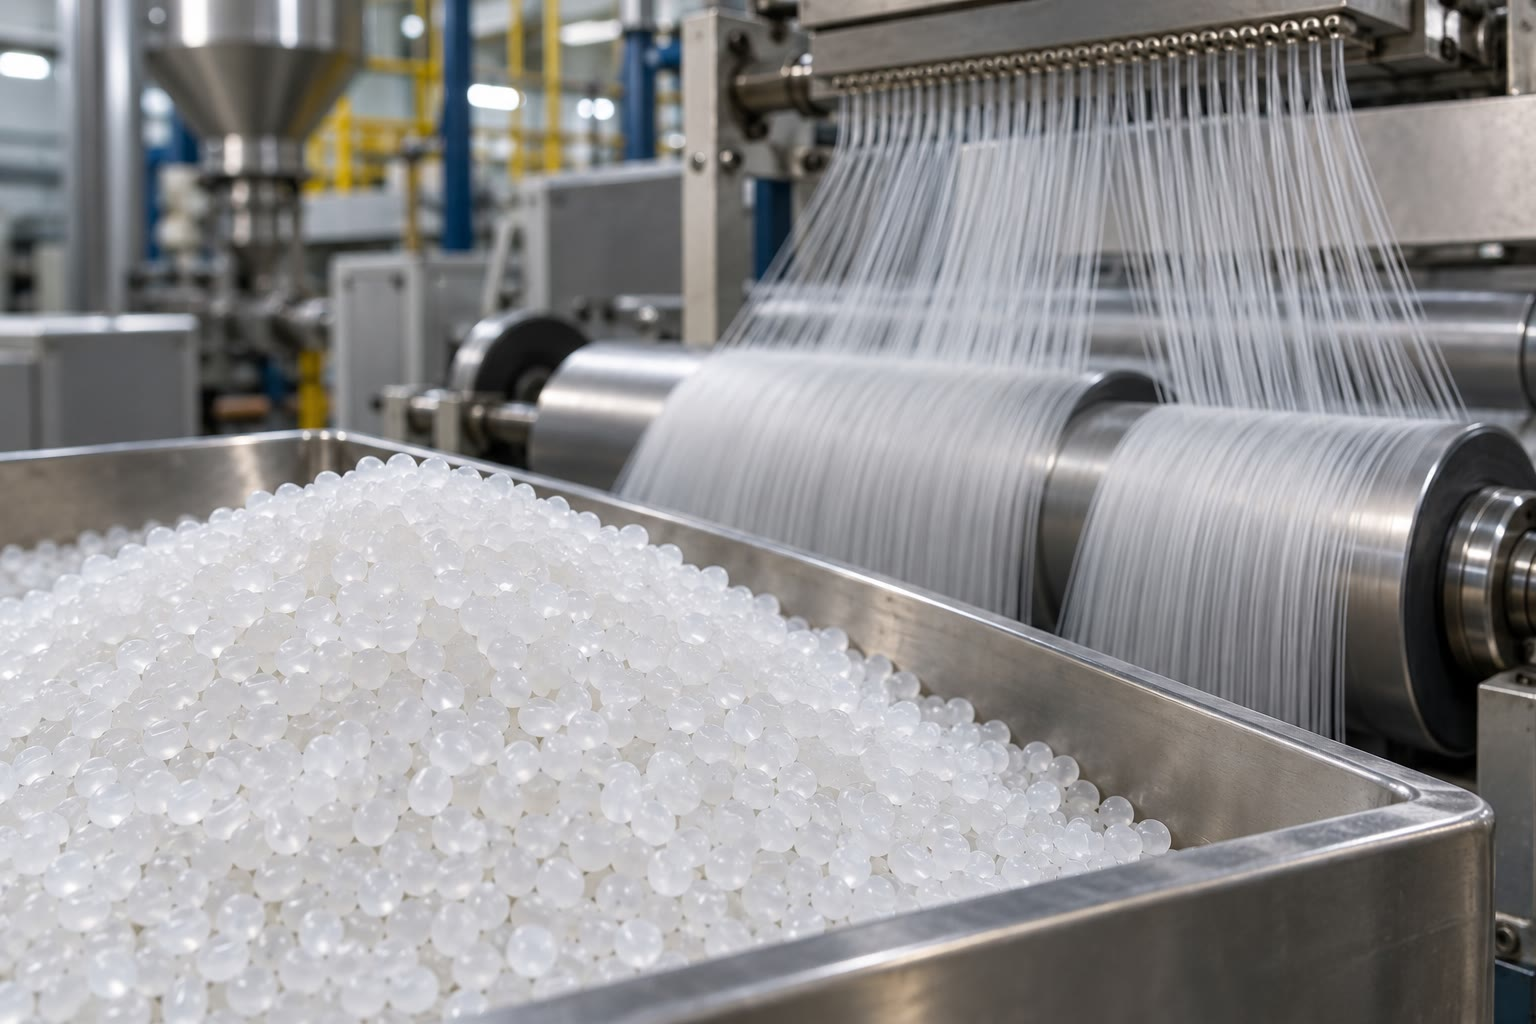
\includegraphics[width=0.58\linewidth]{images/book3/ai/b2-29-pellets.jpg}

{\small Granza de \omterm{def:b2:polymer-synthesis:polymer}{polímero} en una planta, la forma en que se venden los termoplásticos, y fibras que se estiran
desde una hilera sobre rodillos giratorios detrás (ilustración).}
\end{omfigure}

\begin{history}[Un rendimiento del 99~\% no basta]
\begin{minipage}[t]{0.2\linewidth}
\vspace{0pt}
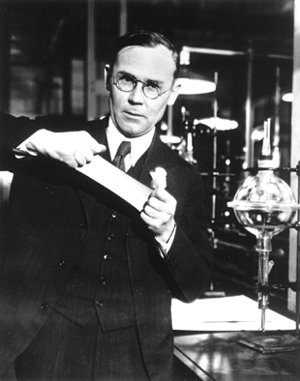
\includegraphics[width=\linewidth]{images/book3/carothers.jpg}
\end{minipage}\hfill
\begin{minipage}[t]{0.76\linewidth}
\vspace{0pt}
Wallace Carothers, un joven profesor universitario contratado por un laboratorio industrial para hacer
investigación fundamental, construyó moléculas largas a partir de reacciones bien conocidas, y sus resultados apoyaron
con fuerza la idea, entonces discutida, de que los \omterm{def:b2:polymer-synthesis:polymer}{polímeros} son moléculas ordinarias, solo que muy largas. Su equipo
obtuvo poliésteres y luego, a partir de 1934, poliamidas; la ecuación que lleva su nombre explica por qué solo
conversiones extremas daban fibras. El nailon entró en producción en 1939. (Fotografía: fotógrafo
desconocido, dominio público; Wikimedia Commons.)
% ledger: hist:polyamides-1934, hist:nylon-production-1939
\end{minipage}
\end{history}

\begin{safety}{\ghs[5mm]{GHS01}\,\ghs[5mm]{GHS02}\,\ghs[5mm]{GHS05}\,\ghs[5mm]{GHS07}\,\ghs[5mm]{GHS08}\,\ghs[5mm]{GHS09}}
El estireno es inflamable y peligroso para la salud. El peróxido de dibenzoílo es un oxidante explosivo cuando está seco y se
conserva húmedo y en frío. La hexano-1,6-diamina y el ácido hexanodioico son corrosivos para los ojos.
% ledger: ghs:styrene, ghs:BPO, ghs:hexanediamine, ghs:adipic-acid
\end{safety}

\section{Ejercicios}

\begin{exercise}[$\star$]\label{exo:b2:polymer-synthesis:1}
Dibújense las \omterm{def:b2:polymer-synthesis:polymer}{unidades de repetición} del polietileno, el polipropileno, el poli(cloruro de vinilo), el poliestireno y el nailon-6,6.
\end{exercise}

\begin{exercise}[$\star$]\label{exo:b2:polymer-synthesis:2}
¿Por etapas o en cadena?: PET a partir de etano-1,2-diol y ácido benceno-1,4-dicarboxílico; poliestireno;
nailon-6,6; poli(metacrilato de metilo); poli(ácido láctico) a partir de ácido 2-hidroxipropanoico.
\end{exercise}

\begin{exercise}[$\star$]\label{exo:b2:polymer-synthesis:3}
Un poliestireno tiene $\bar X_n = 1000$. Calcúlese $\bar M_n$, despreciando los grupos terminales.
\end{exercise}

\begin{exercise}[$\star$]\label{exo:b2:polymer-synthesis:4}
Una cadena de polipropileno dibujada en zigzag plano tiene sus grupos metilo del lado del lector, luego
hacia atrás, luego hacia el lector, luego hacia atrás, y así sucesivamente. Nómbrese su \omterm{def:b2:polymer-synthesis:tacticity}{tacticidad}. ¿Podría cristalizar?
\end{exercise}

\begin{exercise}[$\star\star$]\label{exo:b2:polymer-synthesis:5}
Una muestra es una mezcla de masas iguales de dos fracciones, de masas molares \qty{10}{kg/mol} y
\qty{100}{kg/mol}. Calcúlense $\bar M_n$, $\bar M_w$ y la \omterm{def:b2:polymer-synthesis:averages}{dispersidad}.
\end{exercise}

\begin{exercise}[$\star\star$]\label{exo:b2:polymer-synthesis:6}
Calcúlese $\bar X_n$ para una \omterm{def:b2:polymer-synthesis:step-chain}{polimerización por etapas} equilibrada con $p = 0.98$ y con $p = 0.995$.
\end{exercise}

\begin{exercise}[$\star\star$]\label{exo:b2:polymer-synthesis:7}
Se mezclan un diácido y una diamina con un exceso del 1~\% (en moles) de la diamina. ¿Cuál es el mayor
$\bar X_n$ que puede alcanzarse?
\end{exercise}

\begin{exercise}[$\star\star$]\label{exo:b2:polymer-synthesis:8}
En una polimerización radicalaria se duplica la concentración de iniciador. ¿En qué factor cambian la velocidad de
polimerización y la \omterm{def:b2:polymer-synthesis:chain-length}{longitud de cadena cinética}?
\end{exercise}

\begin{exercise}[$\star\star$]\label{exo:b2:polymer-synthesis:9}
El poli(cloruro de vinilo) es rígido; las mangueras de jardín hechas con él son flexibles porque contienen un plastificante,
una molécula pequeña mezclada entre las cadenas. Explíquese mediante la transición vítrea.
\end{exercise}

\begin{exercise}[$\star\star\star$]\label{exo:b2:polymer-synthesis:10}
Demuéstrese que la distribución másica de Flory $w_x = x(1-p)^2p^{\,x-1}$, vista como función de una variable continua
$x$, es máxima en $x = -1/\ln p$, y que este valor es cercano a $\bar X_n$ cuando $p$ es cercano a 1.
\end{exercise}

\begin{exercise}[$\star\star\star$]\label{exo:b2:polymer-synthesis:11}
El PET se obtiene en dos etapas: el benceno-1,4-dicarboxilato de dimetilo con un exceso de etano-1,2-diol da
benceno-1,4-dicarboxilato de bis(2-hidroxietilo) y metanol; después este diéster se calienta a vacío
y polimeriza, liberando etano-1,2-diol. Escríbanse ambas etapas y explíquese cómo la segunda etapa
resuelve el problema estequiométrico de la ecuación de Carothers.
\end{exercise}

\begin{exercise}[$\star\star\star$]\label{exo:b2:polymer-synthesis:12}
En una copolimerización radicalaria de los \omterm{def:b2:polymer-synthesis:polymer}{monómeros} 1 y 2, la composición instantánea del \omterm{def:b2:polymer-synthesis:copolymer}{copolímero} viene
dada por $\dfrac{\mathrm d[\mathrm M_1]}{\mathrm d[\mathrm M_2]} = \dfrac{[\mathrm M_1](r_1[\mathrm M_1]
+ [\mathrm M_2])}{[\mathrm M_2]([\mathrm M_1] + r_2[\mathrm M_2])}$, donde $r_1$ y $r_2$ son las
razones de reactividad (datos de ejercicio: $r_1 = 2.0$, $r_2 = 0.5$). Calcúlese la razón de unidades en el
\omterm{def:b2:polymer-synthesis:copolymer}{copolímero} formado a partir de una alimentación equimolar. ¿Qué ocurre si $r_1 = r_2 = 0$?
\end{exercise}

\section{Problema: nailon-6,6 por kilos}

\begin{problem}[{Problema de fin de semana --- los monómeros y la sal de nailon, la ecuación de Carothers, un
desequilibrio deliberado, la distribución de Flory y el agua liberada}]
\label{pb:b2:polymer-synthesis:1}
El nailon-6,6 se obtiene a partir de hexano-1,6-diamina y ácido hexanodioico. Los grupos terminales se desprecian en todo el problema.
Masas molares (\unit{g/mol}): C 12.011, H 1.008, N 14.007, O 15.999.
% ledger: aw:C, aw:H, aw:N, aw:O, ghs:hexanediamine, ghs:adipic-acid

\medskip
\noindent\textbf{Parte I --- \omterm{def:b2:polymer-synthesis:polymer}{Monómeros} y \omterm{def:b2:polymer-synthesis:polymer}{unidad de repetición}.}
\begin{enumerate}
  \item Escríbanse las fórmulas de los dos \omterm{def:b2:polymer-synthesis:polymer}{monómeros}.
  \item Escríbase la ecuación de formación de un enlace amida.
  \item Los \omterm{def:b2:polymer-synthesis:polymer}{monómeros} se combinan primero en una sal 1\,:\,1, cristalizada en disolución. ¿Por qué?
  \item Dese la \omterm{def:b2:polymer-synthesis:polymer}{unidad de repetición} del nailon-6,6, su fórmula y su masa molar.
  \item ¿Cuál es la masa molar media $M_0$ de una unidad procedente de un \omterm{def:b2:polymer-synthesis:polymer}{monómero} en la cadena?
  \item ¿Qué cuentan los dos números del nombre ``6,6''?
\end{enumerate}

\medskip
\noindent\textbf{Parte II --- La ecuación de Carothers.}
\begin{enumerate}[resume]
  \item Calcúlense $\bar X_n$ y $\bar M_n$ para $p = 0.98$.
  \item Lo mismo para $p = 0.99$.
  \item Explíquese la observación ``un rendimiento del 99~\% no basta''.
  \item ¿Qué grado de avance da $\bar M_n = \qty{10}{kg/mol}$?
  \item ¿Cómo se lleva en la práctica el grado de avance a valores tan altos?
  \item ¿Por qué deben ser muy puros los \omterm{def:b2:polymer-synthesis:polymer}{monómeros}?
\end{enumerate}

\medskip
\noindent\textbf{Parte III --- Un desequilibrio deliberado.}
\begin{enumerate}[resume]
  \item La diamina se usa con un exceso molar del 1~\%. Calcúlese $r$.
  \item Calcúlense el mayor $\bar X_n$ y el mayor $\bar M_n$ que pueden alcanzarse entonces.
  \item Calcúlese $\bar X_n$ para $p = 0.99$ con este desequilibrio.
  \item ¿Qué grupos terminan las cadenas al final de la reacción?
  \item A veces se añade un poco de ácido etanoico. ¿Qué efecto tiene sobre las cadenas?
  \item ¿Por qué limitaría un fabricante a propósito la longitud de las cadenas?
\end{enumerate}

\medskip
\noindent\textbf{Parte IV --- Distribución y balance de materia.}
\begin{enumerate}[resume]
  \item Para una mezcla equilibrada con $p = 0.99$, dese la \omterm{def:b2:polymer-synthesis:averages}{dispersidad}.
  \item Calcúlese $\bar M_w$ para $p = 0.99$.
  \item Para $p = 0.99$, ¿qué fracción de las moléculas, y qué fracción de la masa, es todavía
        \omterm{def:b2:polymer-synthesis:polymer}{monómero} sin reaccionar?
  \item ¿Cerca de qué longitud de cadena es máxima la distribución másica?
  \item Calcúlese la masa de agua liberada por kilogramo de nailon-6,6.
  \item ¿Por qué el hilado en fundido necesita un $\bar M_n$ dentro de un intervalo?
  \item Indíquese el grado de avance que da $\bar M_n = \qty{20}{kg/mol}$ para una mezcla equilibrada.
\end{enumerate}
\end{problem}
